\subsection{Linear Approximations}\label{sec:LinApprox}
We begin by the first derivative as an application of the tangent line to approximate $f$.

Recall that the tangent line to $f(x)$ at a point $x=a$ is given by
\[ L(x) = f'(a) (x-a) + f(a).\]
The tangent line in this context is also called the \dfont{linear approximation} to $f$ at $a$.

If $f$ is differentiable at $a$ then $L$ is a good approximation of
$f$ so long as $x$ is ``not too far'' from $a$.  Put another way, if
$f$ is differentiable at $a$ then under a microscope $f$ will look
very much like a straight line, and thus will look very much like $L$;
since $L(x)$ is often much easier to compute than $f(x)$, then it makes sense to use $L$ as an approximation. Figure~\ref{fig:linear_approximation} 
shows a tangent line to $\ds y=x^2$ at three different magnifications. 

\figure[!ht]
\centerline{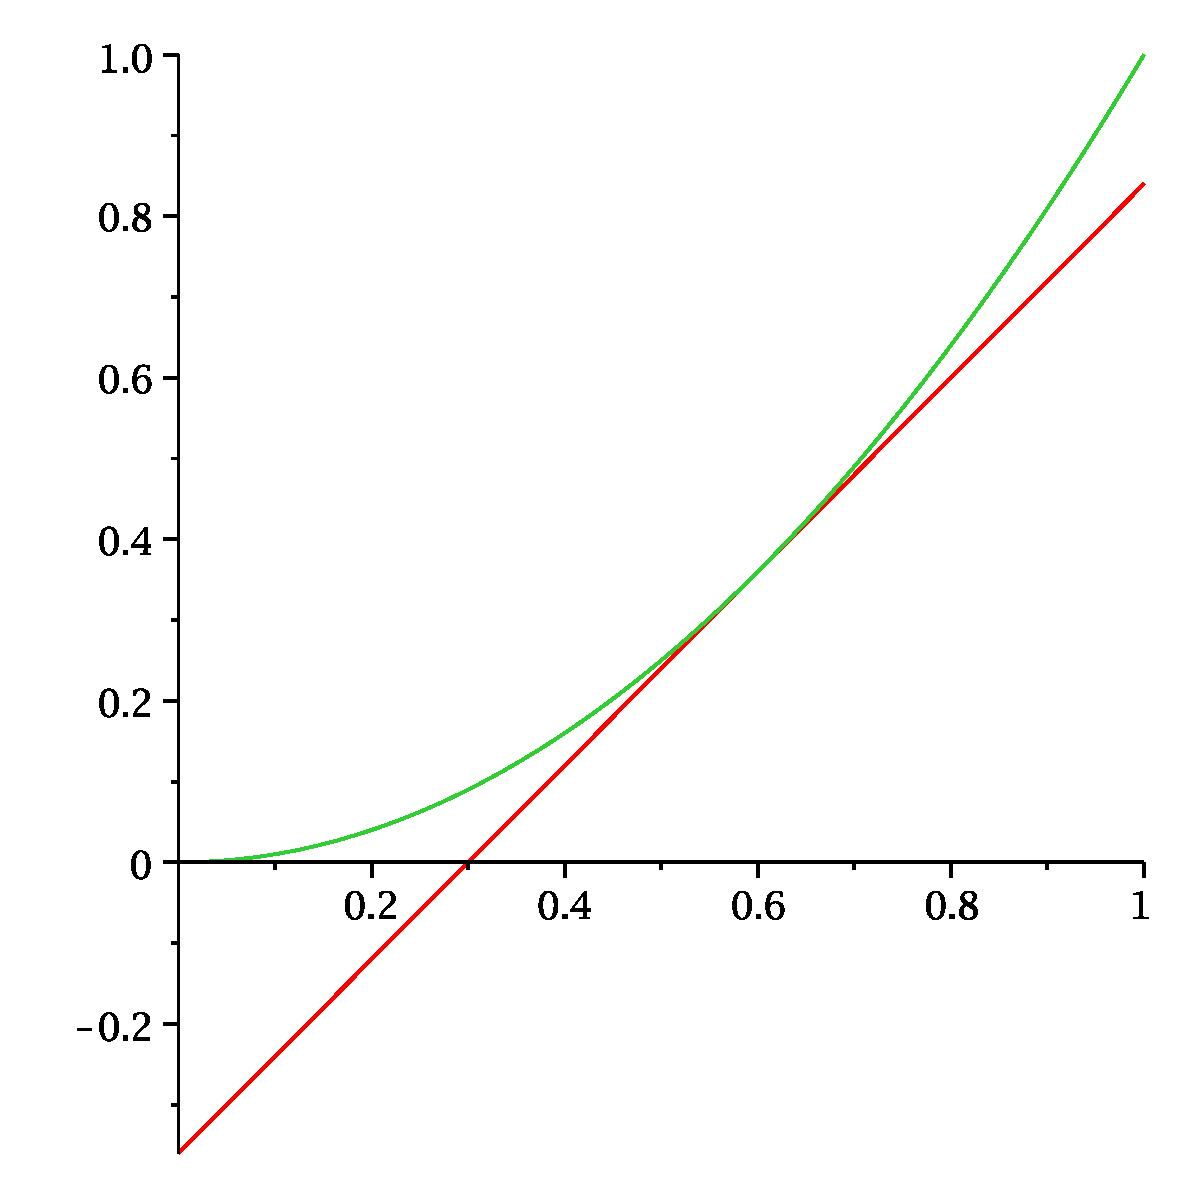
\includegraphics[width=2in]{images/linear_approx_1}\hfill
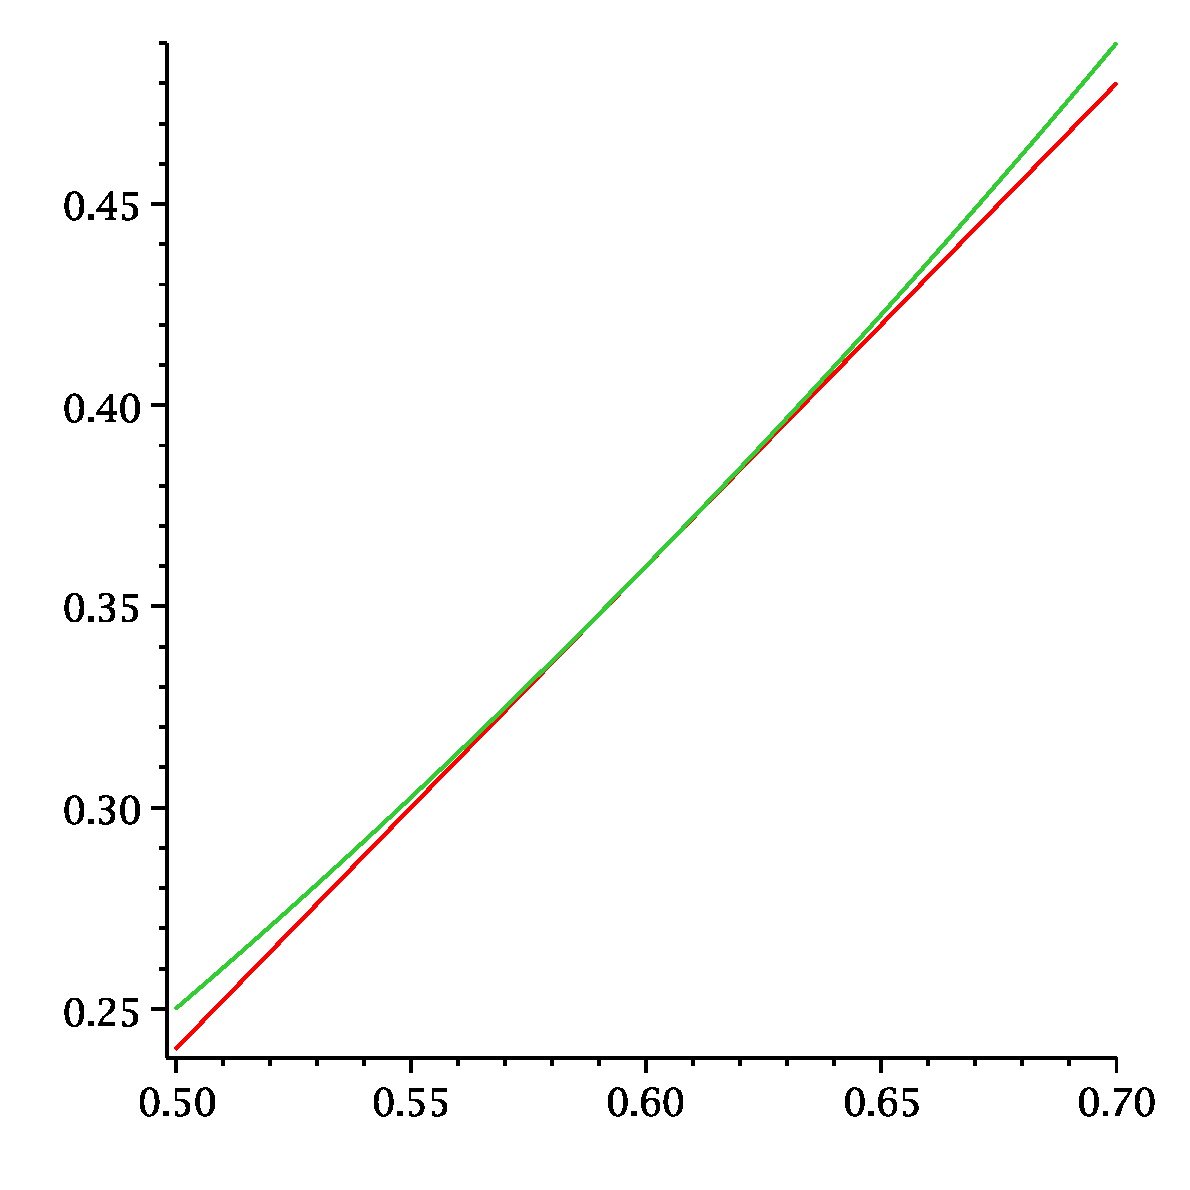
\includegraphics[width=2in]{images/linear_approx_2}\hfill
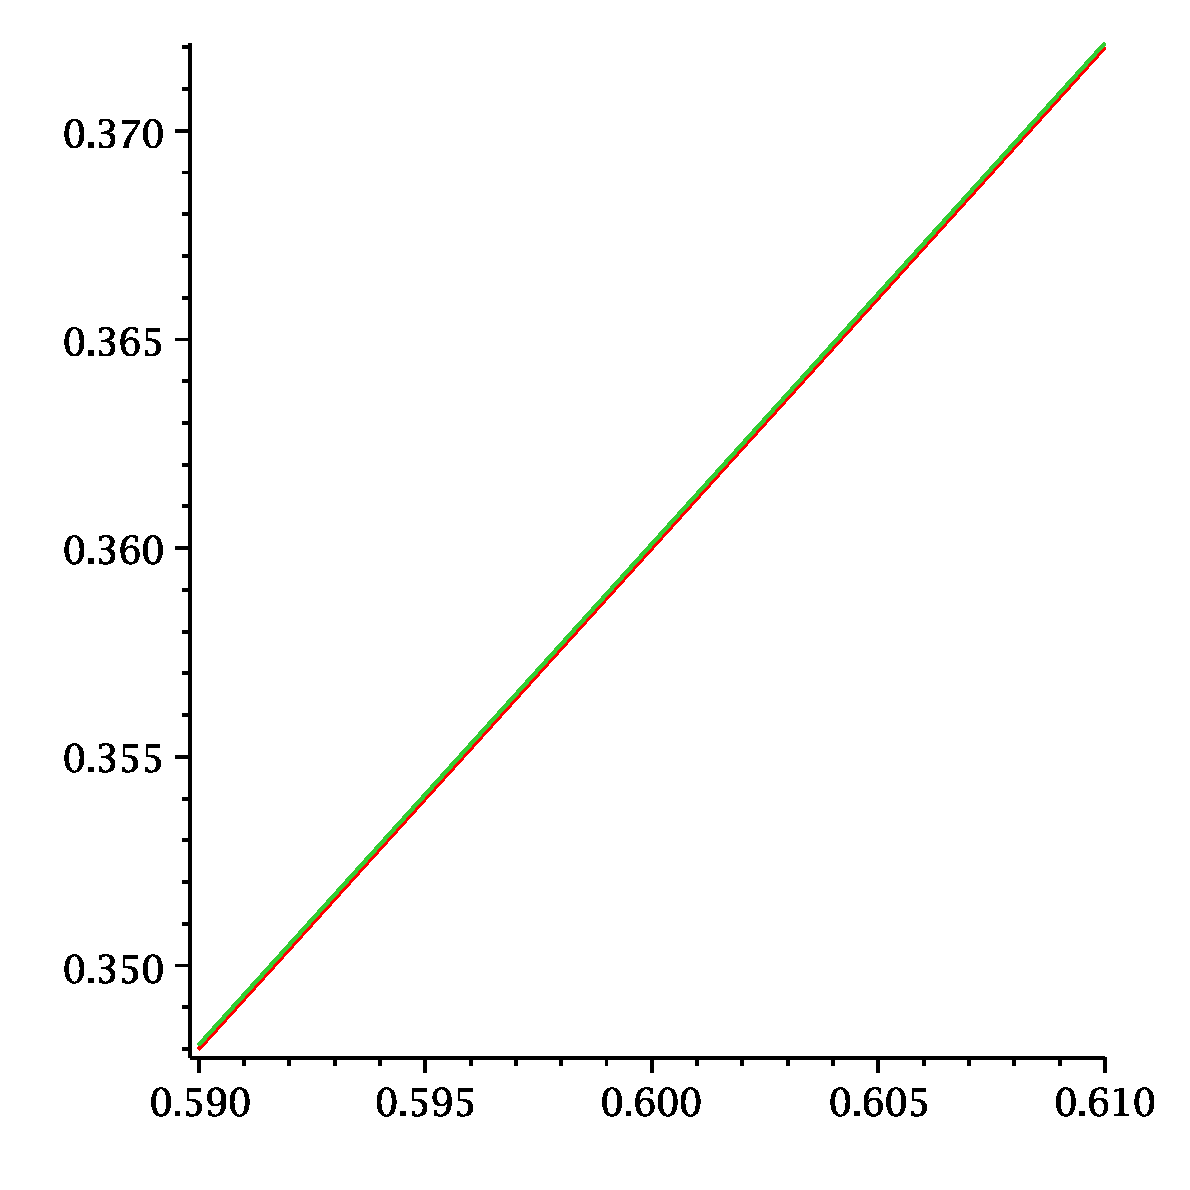
\includegraphics[width=2in]{images/linear_approx_3}\hfill}
\caption{The linear approximation to $\ds y=x^2$. \label{fig:linear_approximation}}
\endfigure

Thus in practice if we want to approximate a difficult value of $f(b)$,
then we may be able to approximate this value using a linear approximation,
provided that we can compute the tangent line at some point $a$ close to $b$.
Here is an example.

\begin{example}{Linear Approximation}{linear approximation}
Let $f(x)=\sqrt{x+4}$, what is $f(6)$?
\end{example}

\begin{solution}
We are asked to calculate $f(6)=\sqrt{6+4}=\sqrt{10}$ which is not easy
to do without a calculator. However 9 is (relatively) close to 10 and
of course $f(5)=\sqrt{9}$ is easy to compute, and we use this to approximate $\sqrt{10}$.

To do so we have $f'(x)=1/(2\sqrt{x+4})$, and thus the linear approximation to $f$ at $x=5$ is
\[L(x)=\bigg(\frac{1}{2\sqrt{5+4}}\bigg)(x-5)+\sqrt{5+4}=\frac{x-5}{6}+3.\]

Now to estimate $\sqrt{10}$, we substitute 6 into the linear approximation $L(x)$ instead of $f(x)$, to obtain
\[ \sqrt{6+4}\approx \frac{6-5}{6}+3=\frac{19}{6}=3\sfrac{1}{6}=3.1\bar{6}\approx 3.17 \]

It turns out the exact value of $\sqrt{10}$ is actually 3.16227766\ldots
but our estimate of 3.17 was very easy to obtain and is relatively accurate.
This estimate is only accurate to one decimal place.
\end{solution}
 
With modern calculators and computing software it may not appear
necessary to use linear approximations, but in fact they are quite
useful. For example in cases requiring an explicit numerical approximation, they
allow us to get a quick estimate which can be used as a
``reality check'' on a more complex calculation. Further in some complex
calculations involving functions, the linear approximation makes an
otherwise intractable calculation possible without serious loss of
accuracy.

\begin{example}{Linear Approximation of Sine}{linear approximation of sine}
Find the linear approximation of $\sin x$ at $x=0$, and use it to compute small values of $\sin x$.
\end{example}

\begin{solution}
If $f(x)=\sin x$, then $f'(x)=\cos x$, and thus the linear approximation of $\sin x$ at $x=0$ is:
\[ L(x)=\cos (0)(x-0)+\sin (0)=x. \]
Thus when $x$ is small this is quite a good approximation and is used
frequently by engineers and scientists to simplify some calculations.

For example you can use your calculator (in radian mode since the
derivative of $\sin x$ is $\cos x$ only in radian) to see that
\[ \sin (0.1)=0.099833416\ldots \]
and thus $L(0.1)=0.1$ is a very good and quick approximation without any calculator!
\end{solution}


%%%%%%%%%%%%%%%%%%%%%%%%%%%%%%%%%%%%%%%%%%%%%%%
\Opensolutionfile{solutions}[ex]
\section*{Exercises for \ref{sec:LinApprox}}

\begin{enumialphparenastyle}

%%%%%%%%%%
\begin{ex} 
Find the linearization $L(x)$ of $f(x)=\ln (1+x)$ at $a=0$. Use
this linearization to approximate $f(0.1)$.
\begin{sol}
$L(x)=x$, $f(0.1)\approx L(0.1)=0.1$
\end{sol}
\end{ex}

%%%%%%%%%%
\begin{ex} 
Use linear approximation to estimate $(1.9)^3$.
\begin{sol}
Choose $f(x)=x^3$ and $a=2$, the closest integer to 1.9. The
linearization of $f$ at $a$ is $L(x)=12(x-2)+8$, and $(1.9)^3=f(1.9)\approx L(1.9)=12(1.9-2)+8=6.8$.
\end{sol}
\end{ex}

%%%%%%%%%%
\begin{ex} 
Show in detail that the linear approximation of
$\sin x$ at $x=0$ is $L(x)=x$ and the linear approximation of $\cos x$
at $x=0$ is $L(x)=1$.
\end{ex}

%%%%%%%%%%
\begin{ex} 
Use $f(x)=\sqrt[3]{x+1}$ to approximate $\sqrt[3]{9}$ by choosing an
appropriate point $x=a$. Are we over- or under-estimating the value of $\sqrt[3]{9}$? Explain.
\begin{sol}
Choose $a=7$ since $f(7)=\sqrt[3]{7+1}=\sqrt[3]{8}=2$ is an integer
close to $\sqrt[3]{9}$. The linearization of $f$ at $a=7$ is
$L(x)=\sfrac{1}{12}(x-7)+2$. Then $f(8)=\sqrt[3]{8+1}=\sqrt[3]{9}\approx L(8)=\sfrac{1}{12}(8-7)+2=2.08\bar{3}$. We are over-estimating $\sqrt[3]{9}$ since $L(x)>f(x)$ for all $x$ around $a=7$.
\end{sol}
\end{ex}

\end{enumialphparenastyle}